\begin{figure}[p]
  \centering
  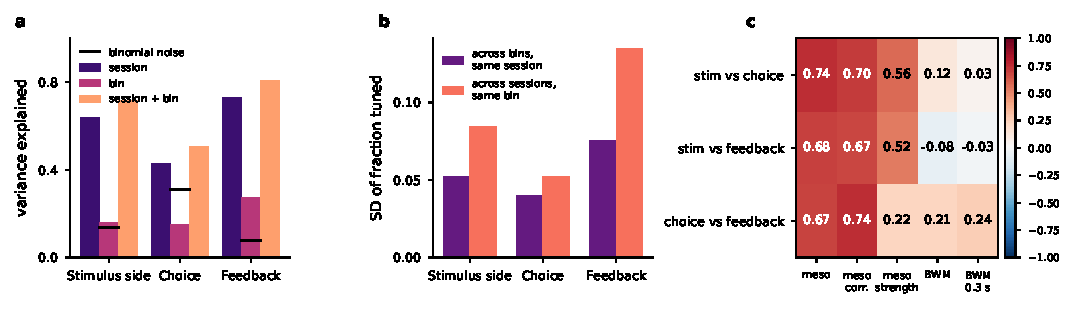
\includegraphics[width=7.00in,height=0.78\textheight,keepaspectratio]{si/si_tuning_variance_panels.pdf}
  \caption{Mesoscope tuning: session vs region effects. Each cell is one session $\times$ one bin (0.4\,mm, hemispheres folded) with $\geq$20 testable neurons. \textbf{a} Variance of the fraction tuned per (session, bin) explained by session means, by bin means and by an additive session + bin model; black ticks: share expected from binomial sampling noise alone (20 or more neurons per cell). \textbf{b} Standard deviation of the fraction tuned across bins of the same session (averaged over sessions) and across sessions recording the same bin (bins with $\geq$3 sessions). \textbf{c} Spearman correlation across bins between the maps of two variables: pooled fraction tuned (as in the main figure), the session-corrected bin effects of the additive model, the median tuning strength, and the BWM pooled fractions with the BWM windows and with the 0.3\,s mesoscope windows.}
  \label{fig:si_tuning_variance}
\end{figure}
